\documentclass{beamer}
\usepackage[utf8]{inputenc}
\usepackage{fontspec}
\usepackage{amsfonts,amsmath,amssymb}
\usepackage{url}
\usepackage{units}
\usepackage{xcolor}
\setmainfont{Liberation Serif}

\definecolor{drkgreen}{RGB}{59,107,0}
\newcommand{\pro}[1]{\textcolor{drkgreen}{#1}}
\newcommand{\con}[1]{\textcolor{red}{#1}}

\usetheme{Warsaw}
\useoutertheme{infolines}
\useinnertheme{rectangles}
\usecolortheme{beaver}
\setbeamerfont{title}{family=\rm}
\AtBeginSection[]
{
  \begin{frame}
    \frametitle{Table of Contents}
    \tableofcontents[currentsection]
  \end{frame}
}


\title{VFPIX Silicon Telescope \\ Custom Electronics \& DAQ Design}
\author[C. Fangmeier]{Caleb Fangmeier}
\institute[UNL]{Univ.\ of Nebraska \-- Lincoln}
\date{August 31, 2015}

\begin{document}

\begin{frame}[plain]
  \titlepage
  \addtocounter{framenumber}{-1}
\end{frame}


\begin{frame}{Table of Contents}
  \tableofcontents
\end{frame}

\section{System Overview}
\begin{frame}{Telescope Block Diagram}
  \centering
  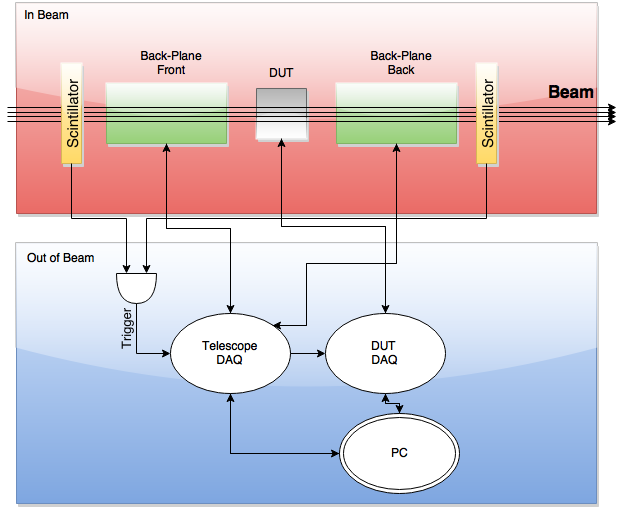
\includegraphics[height=0.8\textheight]{figures/Telescope_Hierarchy}
\end{frame}


\begin{frame}{The Back Plane Board}
  \centering
  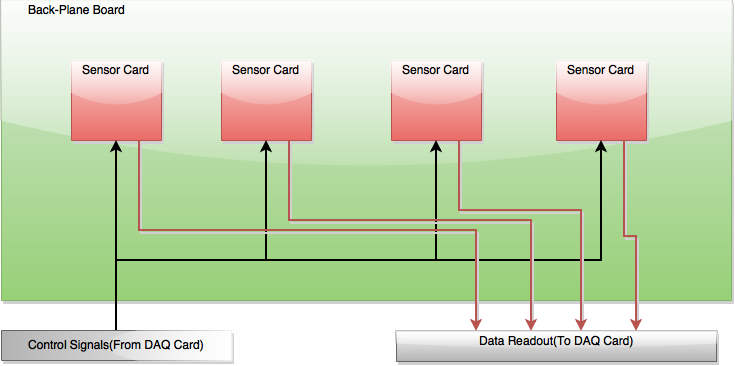
\includegraphics[width=1.0\textwidth]{figures/Telescope_BPB}
\end{frame}

\begin{frame}{The Back Plane Board(Previous Iteration)}
  \centering
  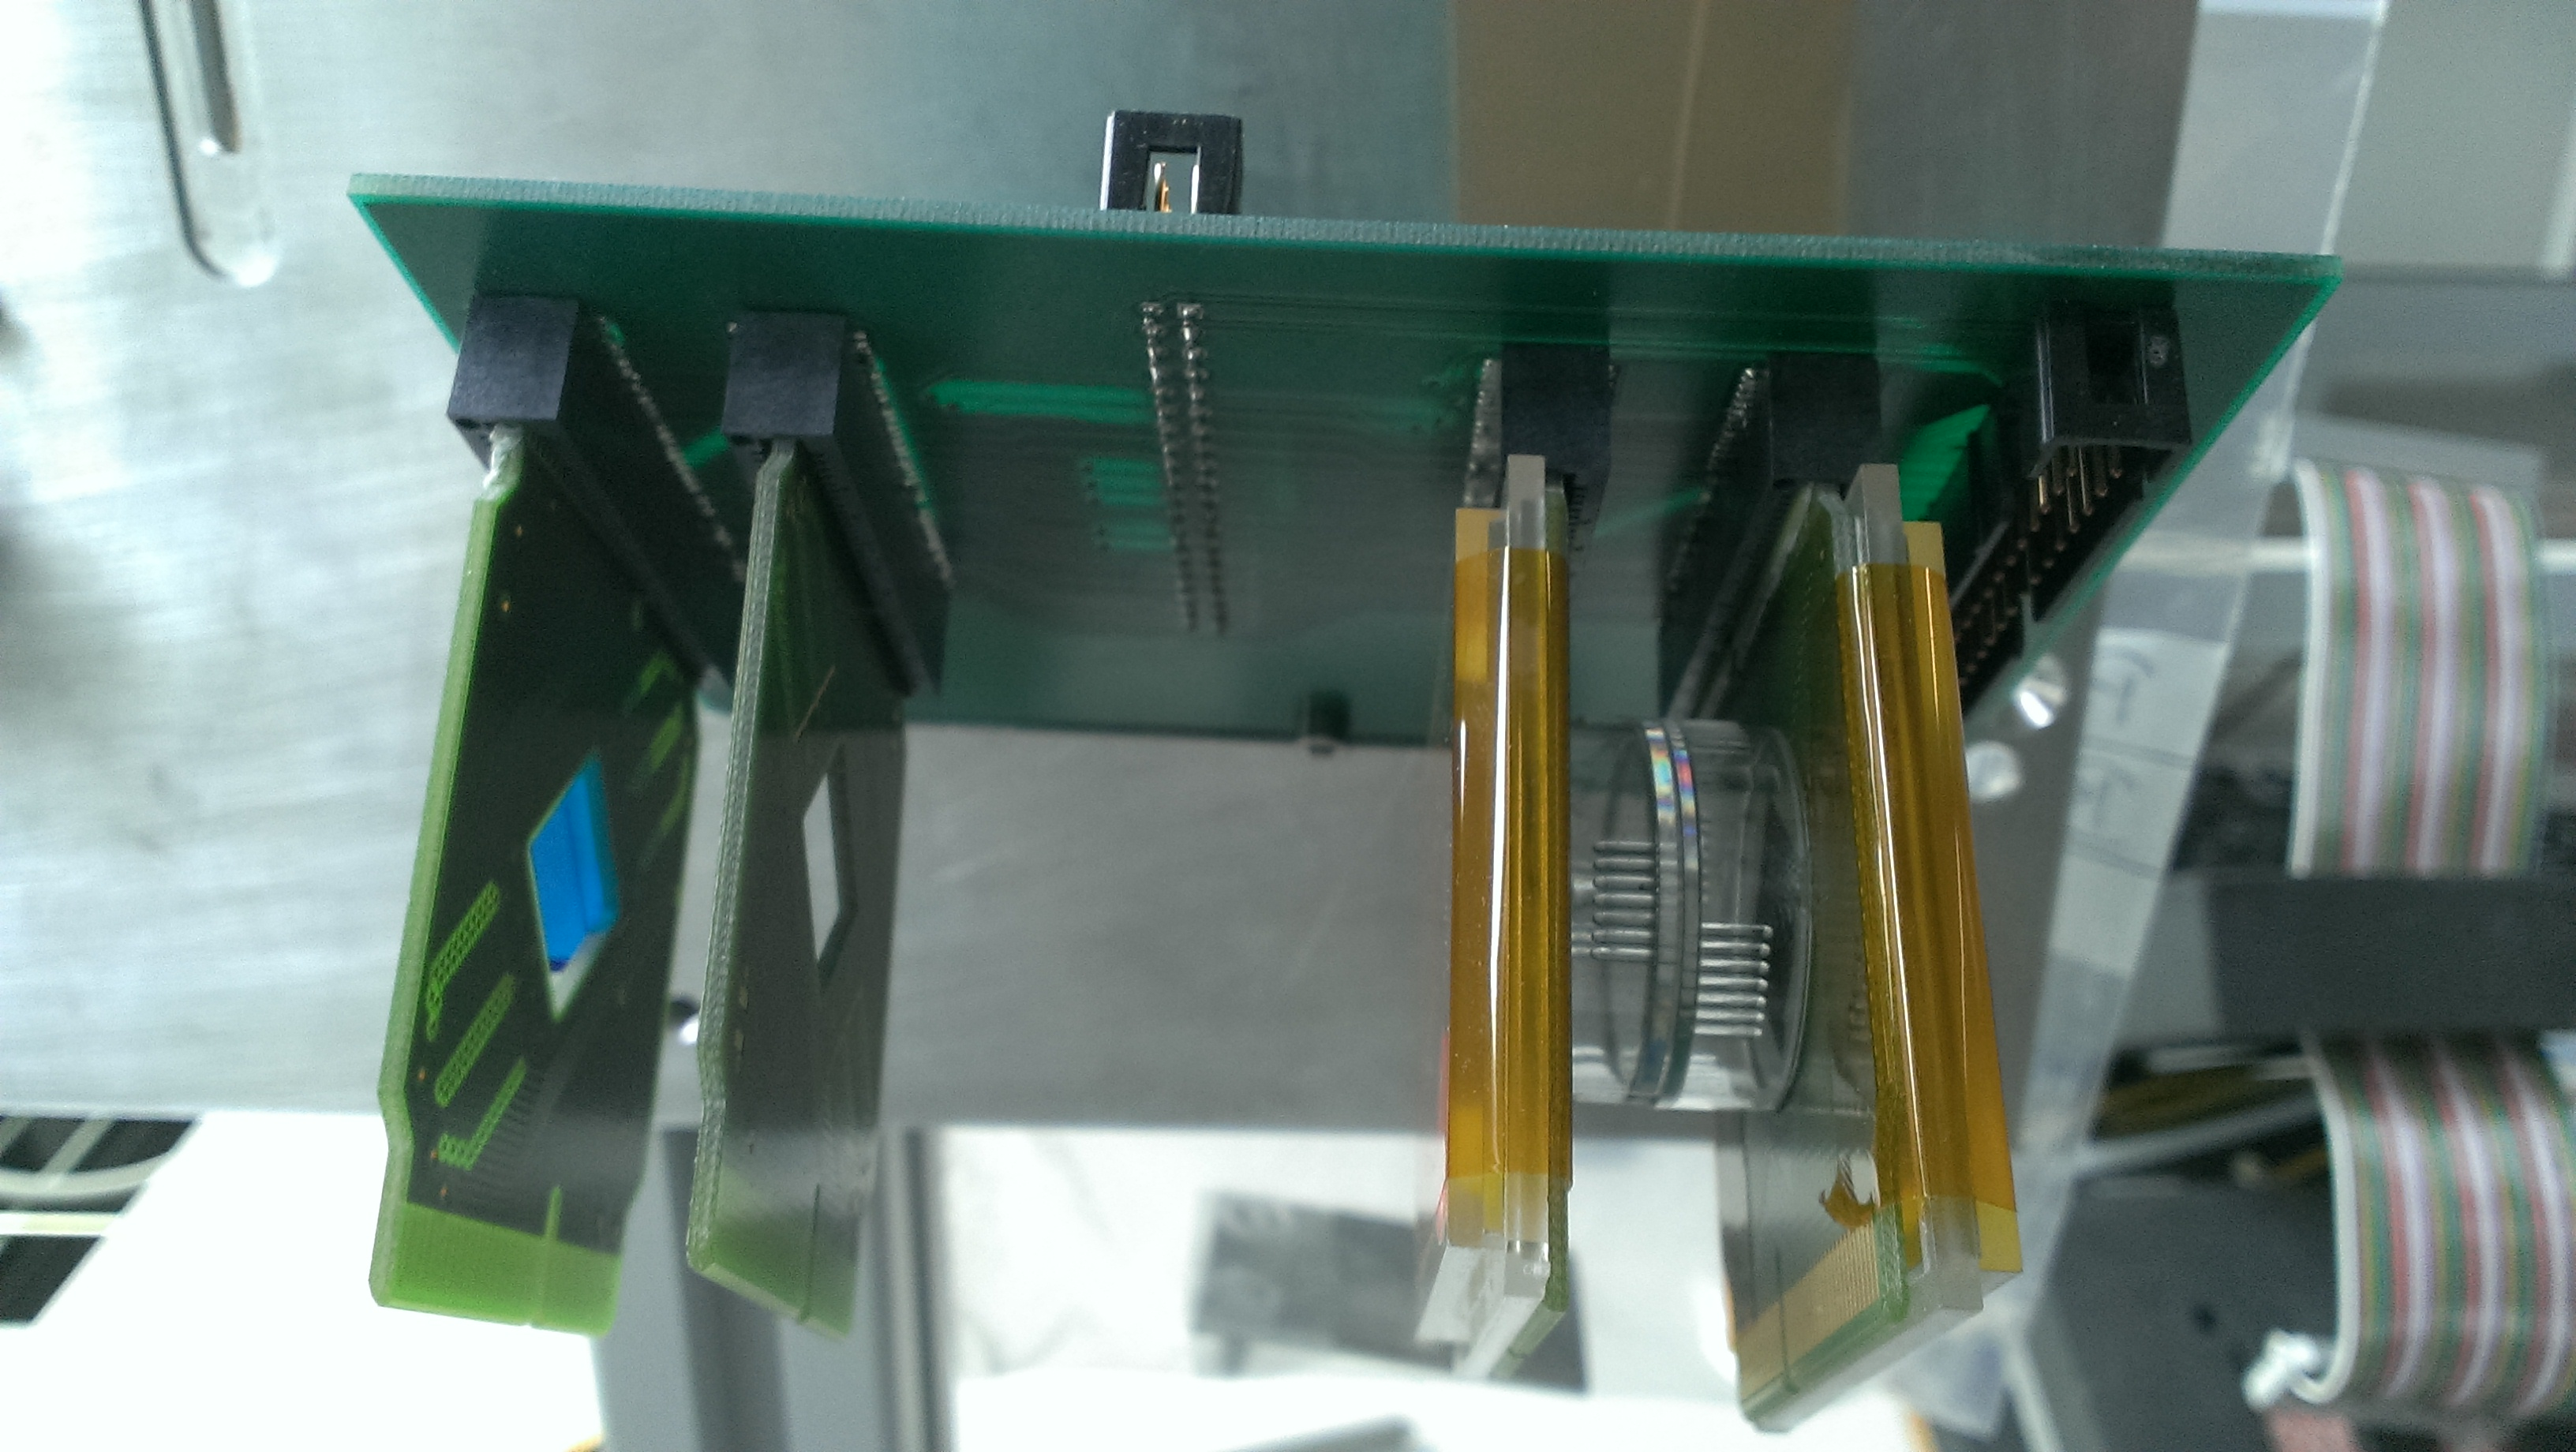
\includegraphics[width=1.0\textwidth]{figures/BPB_Prev}
\end{frame}


\section{Constraints and Freedoms}
\begin{frame}
  \textbf{What parts of the system are fixed?}
  \begin{itemize}
    \item Type and number of Micro-Strip Sensors
    \item APC128 Readout Chip
    \item Testbeam Constraints
      \begin{itemize}
        \item Radiation Exposure
        \item Mechanical Sizes
      \end{itemize}
  \end{itemize}
\end{frame}


\begin{frame}{Micro-Strip Sensor}
  \centering
  \begin{columns}
    \column{0.5\textwidth}
    \begin{itemize}
      \item 512 Strips per Sensor
      \item Adjacent Strips read out on opposite sides by APC128 Chips
    \end{itemize}
    \column{0.5\textwidth}
      \begin{figure}
        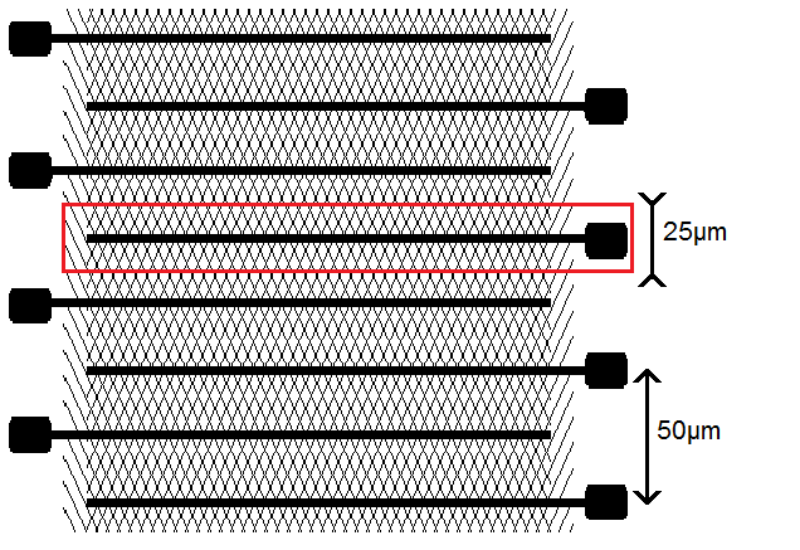
\includegraphics[width=0.9\textwidth]{figures/Microstrip_Sensor}
      \end{figure}
  \end{columns}
\end{frame}

\begin{frame}{Analog Pipeline Chip 128}
  \centering
  \begin{figure}
    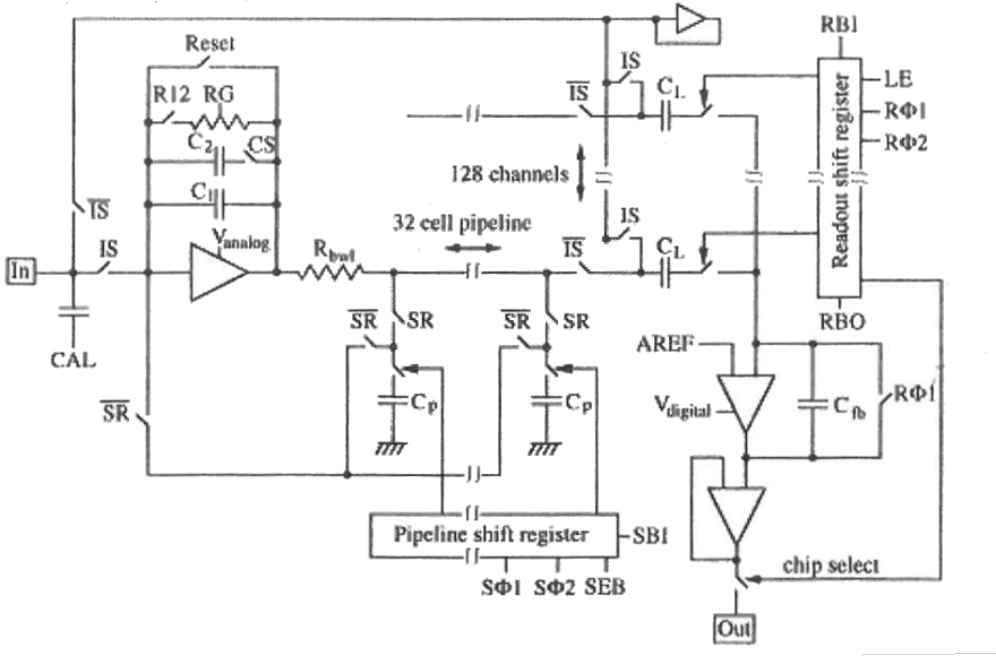
\includegraphics[width=0.9\textwidth]{figures/APC128_Schematic}
  \end{figure}
\end{frame}


\begin{frame}{Analog Pipeline Chip 128}
  \centering
  \begin{columns}
    \column{0.5\textwidth}
      \begin{figure}
        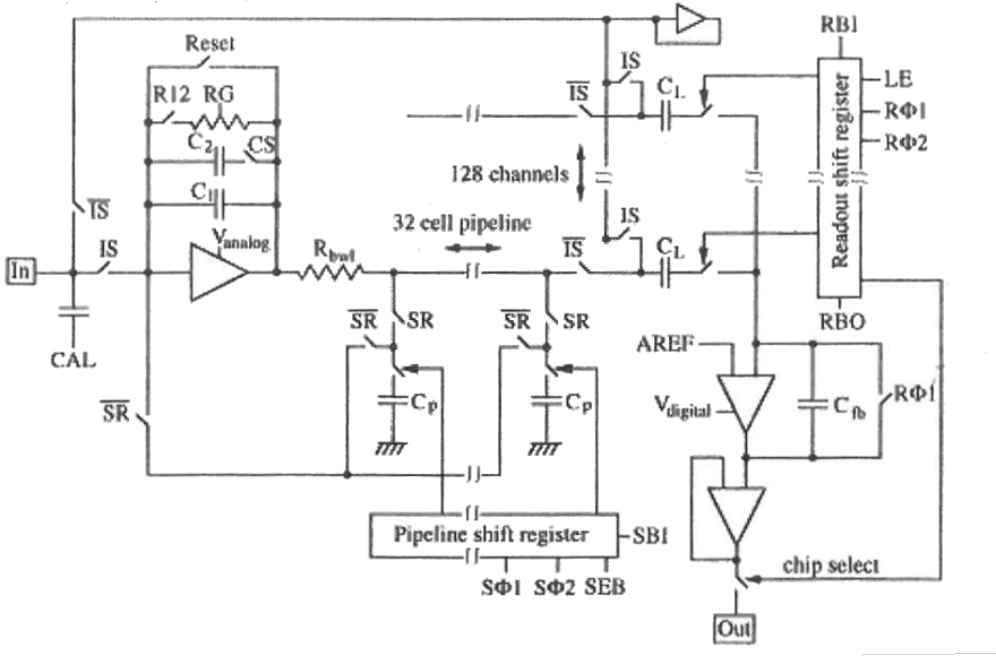
\includegraphics[width=0.95\textwidth]{figures/APC128_Schematic}
      \end{figure}
    \column{0.5\textwidth}
      \begin{figure}
        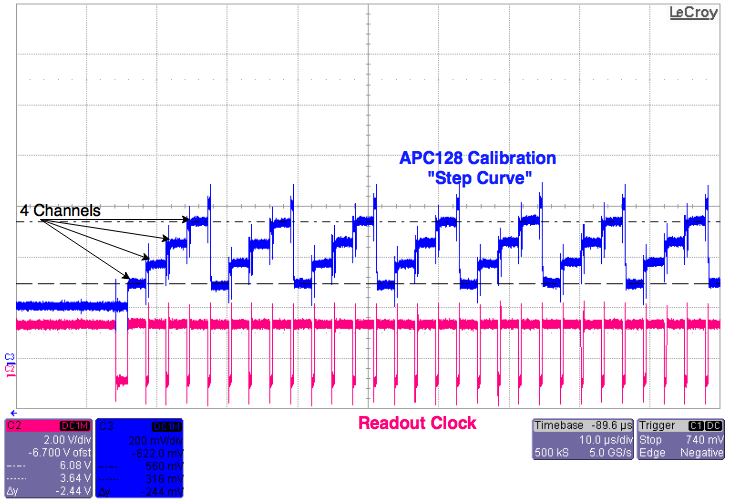
\includegraphics[width=0.95\textwidth]{figures/APC_Readout}
      \end{figure}
  \end{columns}
\end{frame}


\subsection{}
\begin{frame}
  \textbf{What parts are flexible?}
  \begin{itemize}
    \item ADC location, precision(bitness), and sample rate
    \item Cabling
    \item Number/type of readout channels(Serial/Parallel, Analog/Digital)
    \item Digital Controller(FPGA,CPLD,Microcontroller, \dots)
    \item Amplifiers, DACs, Capacitors, Resistors, \dots
    \item PCB layouts of all boards including
      \begin{itemize}
        \item Sensor Mount Card
        \item Back-Plane Board
        \item DAQ Card
      \end{itemize}
  \end{itemize}
\end{frame}


\section{Datarates, Analog vs. Digital Domain}
\begin{frame}
  \begin{itemize}
    \item 8 Sensors * 512 Strips/Sensor = 4096 Strips
    \item Each APC128 serializes 128 Strips
    \item $\rightarrow$ 32 Analog Channels with 128 Strips/Channel
    \item More serialization $\rightarrow$ fewer cables/ADCs, but slower readout
    \item Faster readout is critical to data rate!
  \end{itemize}

  \vspace{0.5 in}
  \begin{center}
    \huge \emph{Where to Digitize?}
  \end{center}
\end{frame}


\begin{frame}
  \centering
  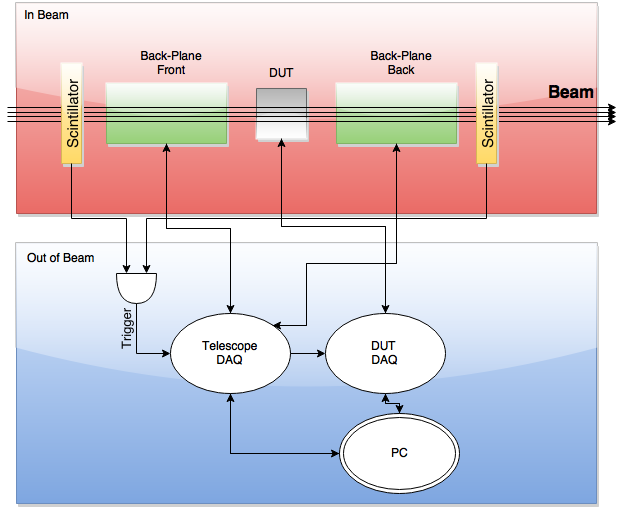
\includegraphics[height=0.8\textheight]{figures/Telescope_Hierarchy}
\end{frame}


\begin{frame}
  \begin{itemize}
    \item Any stateful electronics(e.g. ADCs, DACs, RAM, etc.) must be out of beam to avoid SEUs.
    \item Op-amps and other linear electronics are OK.
    \item However, less distance between sensor and ADC means less noise and, potentially, faster readout.
    \item Compromise is to place ADC on DAQ board $\approx$\unit{0.5}{m} from telescope, but out of beam.
  \end{itemize}
\end{frame}

\section{Parts Selection}
\begin{frame}{APC128 Buffer/Line Driver}
  \centering
  \begin{itemize}
    \item Previous designs required APC128 to drive signal line directly.
    \item APC128 output very weak. $\approx$ \unit{800}{$\Omega$} output impedance.
    \item Cable capacitance resulted in slow rise times.
    \item Place buffer amp close to APC128
  \end{itemize}
  \textbf{Choice of amp is the Analog Devices AD8138}
  \begin{itemize}
    \item Very low noise, \unit{5}{nV}/$\sqrt{Hz}$
    \item Appropriate bandwidth(\unit{300}{MHz}) \& slew rate(\unit{1150}{V/$\mu$s})
    \item Differential output suitable for sending down a high-speed cable. e.g. CAT-5
  \end{itemize}
\end{frame}

\begin{frame}[shrink]{ADC}
  \centering
  \textbf{Choice of ADC is the Analog Devices AD9219}
  \begin{figure}
    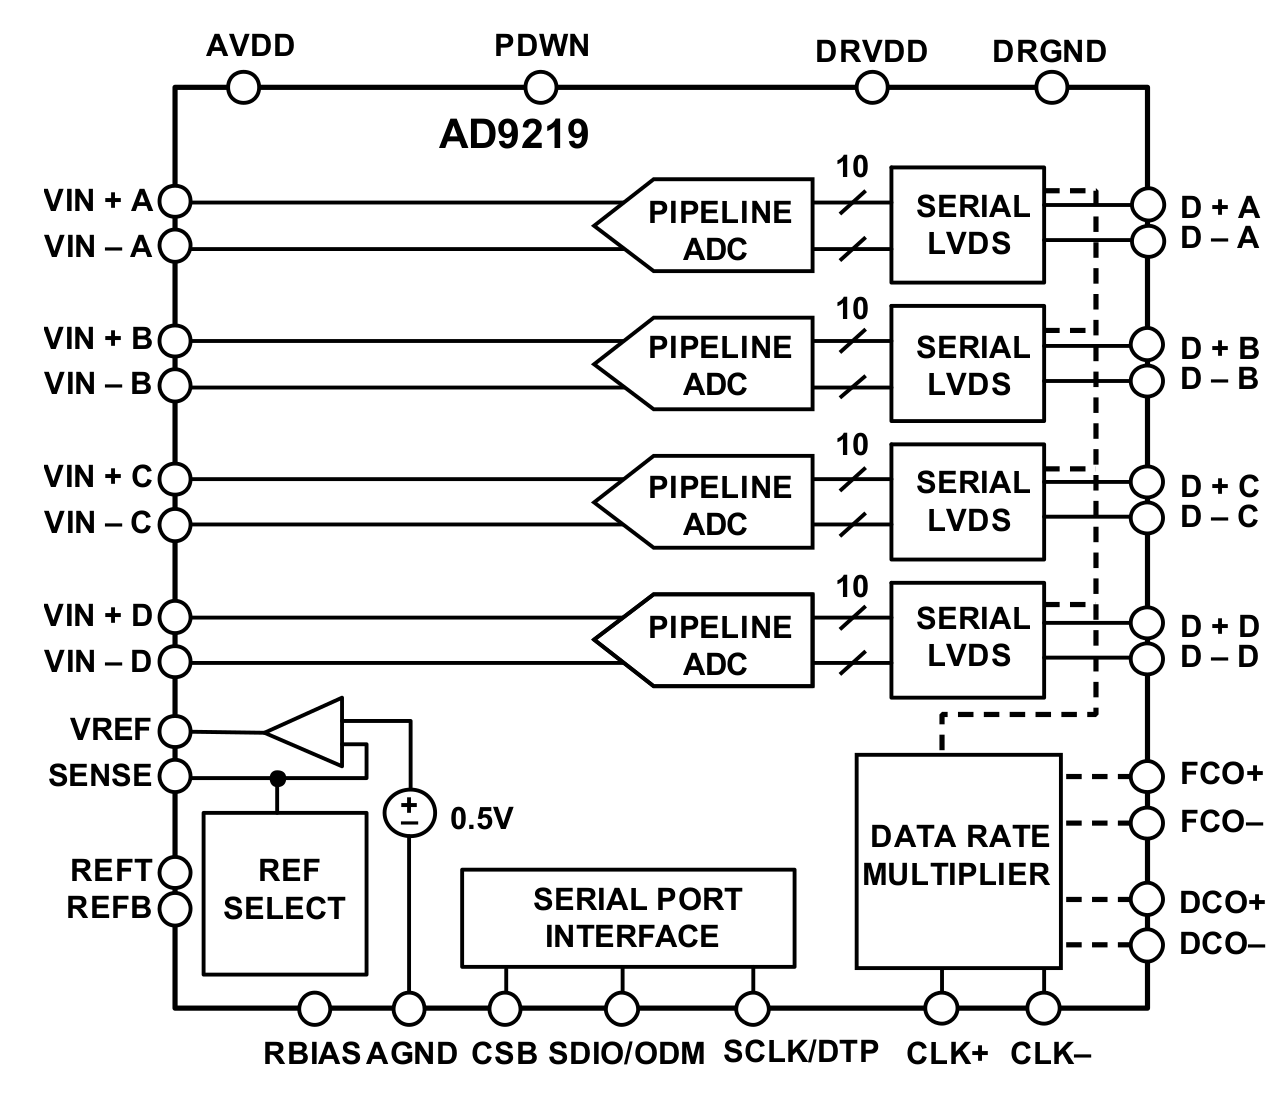
\includegraphics[height=0.4\textheight]{figures/AD9219}
  \end{figure}
  \begin{itemize}
    \item Sample speed up to 40MHz(will plan on oversampling signal)
    \item 10-bit precision
    \item 4-Channel differential inputs
    \item Requires a clock at sample frequency. Generates own readout clock.
    \item Must optimize PCB environment to achieve maximum performance.
  \end{itemize}
\end{frame}


\begin{frame}[shrink]{Controller}
  \centering
  \textbf{Choice of Controller is Opal Kelly ZEM4310}
  \begin{figure}
    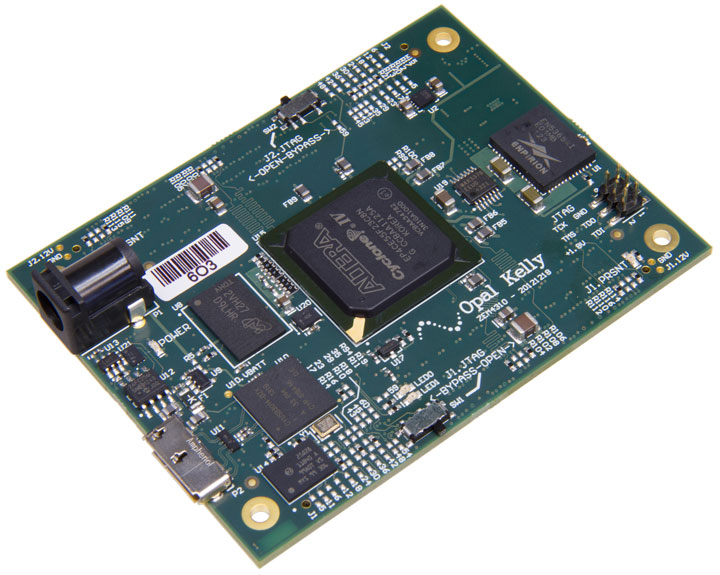
\includegraphics[height=0.35\textheight]{figures/zem4310}
  \end{figure}
  \begin{itemize}
    \item Integrated Module including
      \begin{itemize}
        \item Altera Cyclone IV FPGA
        \item USB 3.0
        \item 128 MiB DDR2 SDRAM
        \item 2xHSMC Expansion Header(on back)
      \end{itemize}
    \item Appropriate for deserializing all 32 ADC channels in parallel
    \item Helps avoid design of difficult and expensive custom FPGA board
  \end{itemize}
\end{frame}


\begin{frame}{General Comments}
  \begin{itemize}
    \item The design must incorporate parts one can actually order.
    \item Digikey is your friend!
    \item Keep a Bill-of-Materials with specific part numbers.
    \item Get used to reading datasheets.
  \end{itemize}
\end{frame}


\begin{frame}{PCB Design Gotchas}
  \begin{itemize}
    \item Make sure the device pinout matches what you think it is. Sometimes multiple parts share a datasheet.
    \item There is no charge for extra writing on the silkscreen. \emph{Use it!}
    \item Check part's datasheet for a recommended PCB footprint. Don't trust the built-in footprint library!
    \item Give some thought to how the board will be assembled.\ e.g. Avoid SMT parts on both sides.
    \item Respect the design rules of your PCB house.\ e.g. Min trace/via sizes
    \item Calculate power requirements and give yourself a 2x safety factor with your supplies.
  \end{itemize}
\end{frame}

\section{PCB Examples}
\begin{frame}{NIM-TTL Level Translator Board}
  \begin{figure}
    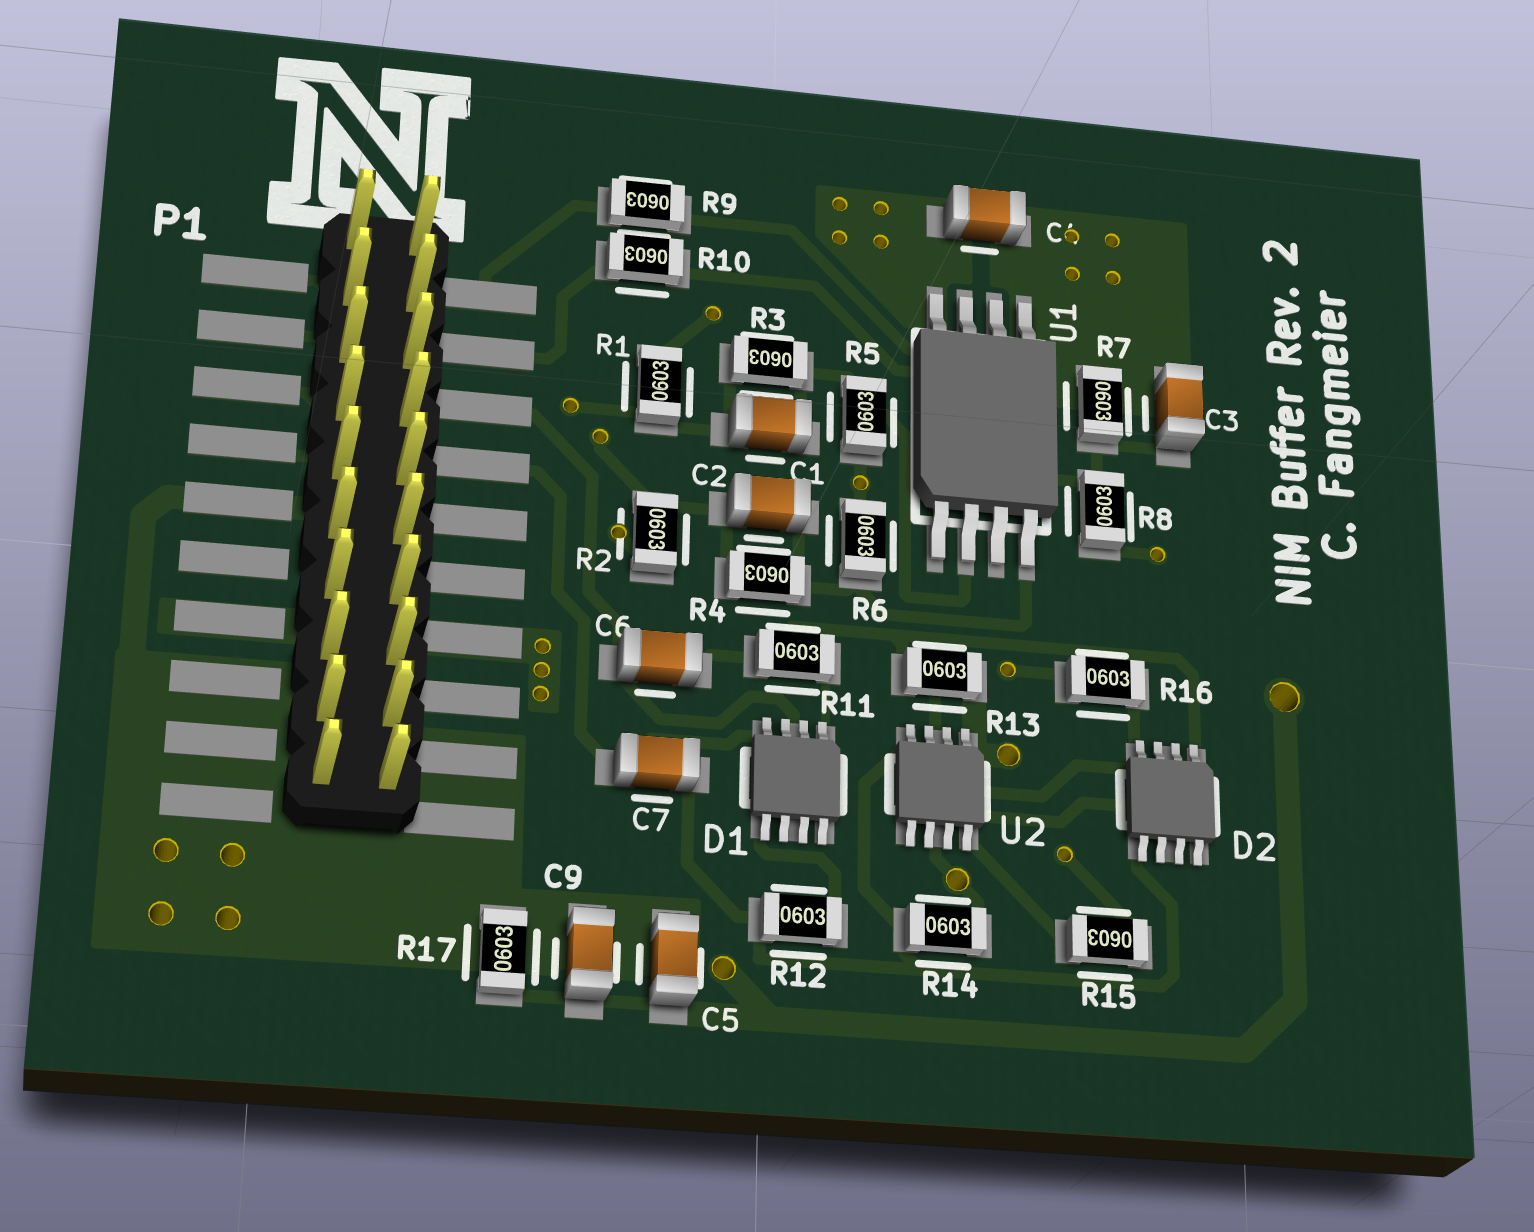
\includegraphics[height=0.8\textheight]{figures/NIM-LTB}
  \end{figure}
\end{frame}
\begin{frame}{APC128 Testboard}
  \begin{figure}
    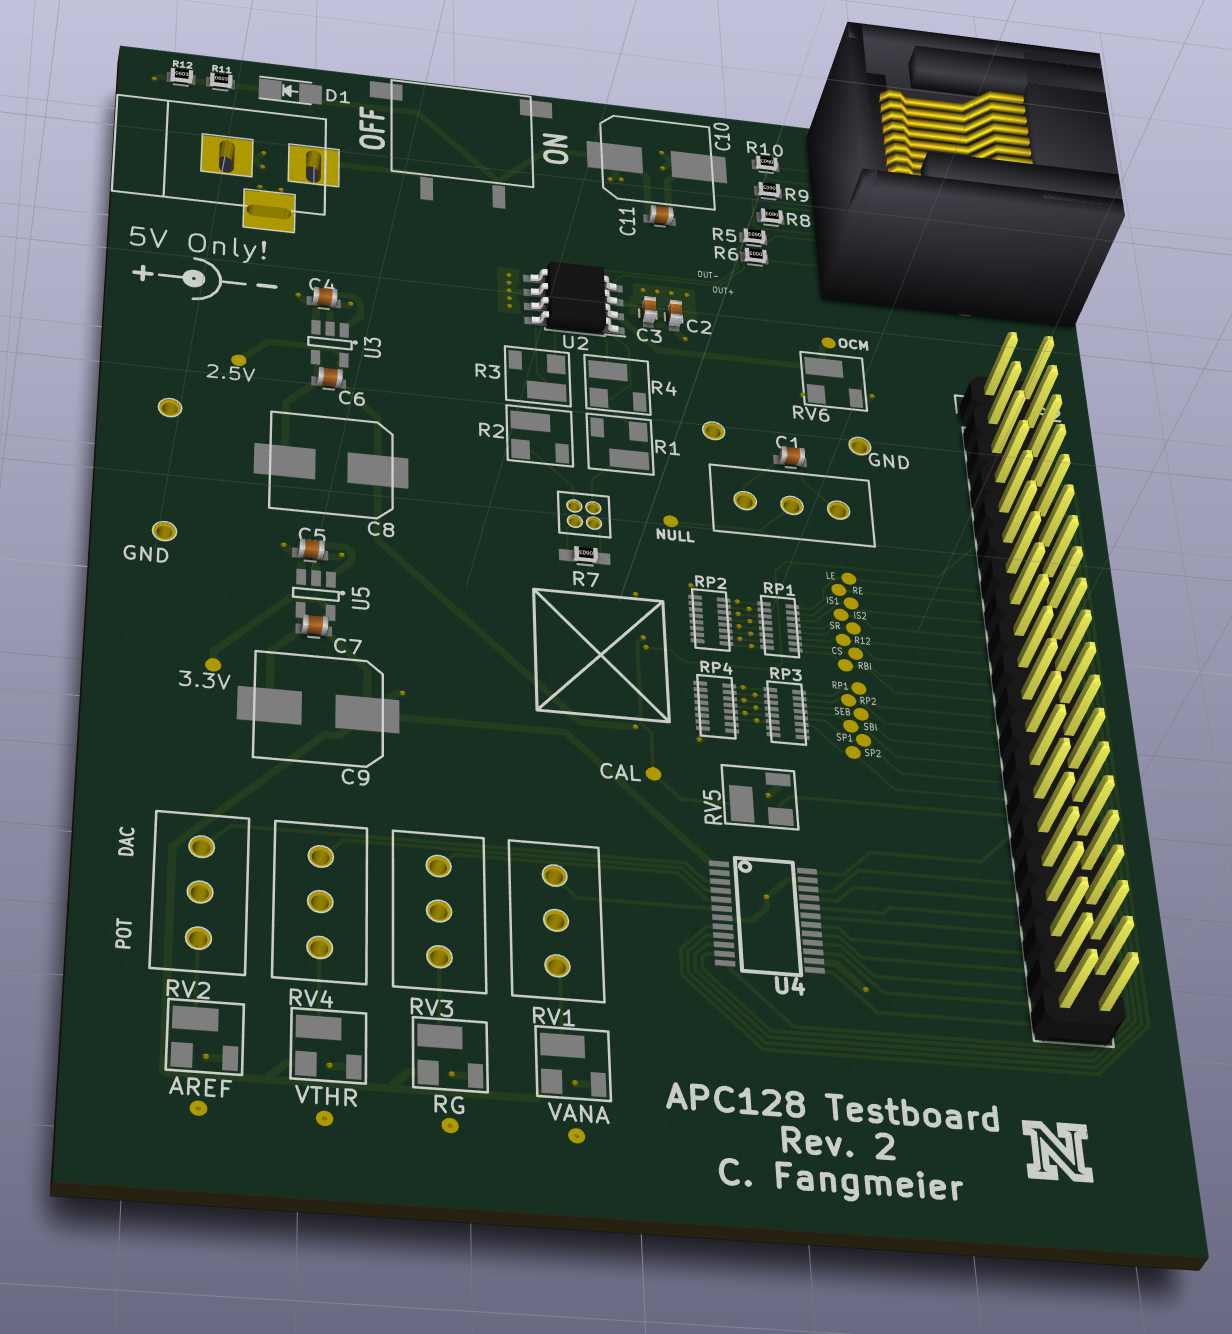
\includegraphics[height=0.8\textheight]{figures/APC128-Testboard}
  \end{figure}
\end{frame}


\section{Software Tools}
\begin{frame}
  \begin{itemize}
    \item \emph{Electronic Simulation} \-- \textbf{QUCS}
      \begin{itemize}
        \item \pro{Free \& Open Source}
        \item \pro{Great support for Linux.}
        \item \pro{Intuitive UI, Integrated Simulation Views}
        \item \pro{Good Support for Generic Simulation}
        \item \con{Poor Integration of Spice Models}
      \end{itemize}
    \item \emph{Circuit Design \& PCB Layout} \-- \textbf{KiCAD}
      \begin{itemize}
        \item \pro{Free \& Open Source}
        \item \pro{No Limit on Board Size or Number of Layers}
        \item \pro{Under Active Development}
        \item \con{Lacks some advanced features of commercial software}
      \end{itemize}
    \item \emph{FPGA Design} \-- \textbf{Quartus II}
      \begin{itemize}
        \item \con{Proprietary}
        \item \pro{Developed By Altera (Same Company as FPGAs)}
        \item \pro{Can Develop Firmware Either Graphically with Block Diagrams or with an HDL (e.g. Verilog)}
      \end{itemize}
  \end{itemize}
\end{frame}

\begin{frame}{Custom Tools}
  \begin{itemize}
    \item \textbf{PatternGen}
      \begin{itemize}
        \item A Tool for converting ASCII waveform files to Verilog
        \item Useful for generating multi-channel bit patterns with an FPGA
      \end{itemize}
    \item \textbf{Make\_Mapping}
      \begin{itemize}
        \item A tool for mapping pins along a connection chain
      \end{itemize}
  \end{itemize}
  \vspace{0.5in}
\end{frame}

\section{}
\begin{frame}{References}
  All custom tools available here: \url{https://github.com/cfangmeier/Small}
  \vspace{.2in}
  \hline
  \vspace{.2in}
  All Circuit/PCB Designs available here: \url{https://github.com/frmeier/VFPIX-telescope-PCB}
\end{frame}

\end{document}
